% PINK reproduction, figure by figure - build with xelatex.
%
%     cd presentation && ./build_pink.sh
%
% Third deck in the set. CGCNN_presentation.tex explains CGCNN;
% ALIGNN_PINK_presentation.tex explains ALIGNN and the findings; this one walks
% the PINK paper's own figures and shows our reproduction of each, plus the
% classification results and the physics written out in full.
%
% Every figure inserted here is either an existing results/ artefact or is
% generated by make_pink_figures.py / make_alignn_figures.py. Nothing is
% redrawn by hand and nothing stands in for a figure we do not have - see the
% "what cannot be reproduced" slide.
\documentclass[aspectratio=169]{beamer}
% Custom beamer theme for the CGCNN presentation.
% ================================================
%
% Kept separate from the content file so the visual system - colours, fonts,
% the card/eyebrow building blocks - can be read and adjusted in one place
% without wading through forty frames of prose.
%
% DESIGN
% ------
% Georgia for headings (a serif with the same weight/character as the
% Cambria used in the project's other teaching decks), Avenir Next for body
% text (same role as their Calibri). Both are macOS system fonts, loaded via
% fontspec, so this MUST be built with xelatex or lualatex - not pdflatex.
%
% Cards are TikZ nodes with `text width` set and NO fixed height. That one
% choice eliminates an entire class of bug: a fixed-height text box that
% silently overflows its frame is exactly what an earlier (PowerPoint)
% version of this deck kept getting wrong. A TikZ node sized only by its
% content cannot overflow itself - it grows to fit, by construction.

\usepackage{fontspec}
\setmainfont{Avenir Next}
\setsansfont{Avenir Next}
\newfontfamily\headingfont{Georgia}
\newfontfamily\monofont{Menlo}

\usepackage{tikz}
\usetikzlibrary{arrows.meta,positioning,shapes.geometric,calc,backgrounds,fit}
\usepackage{amsmath,amssymb}
\usepackage{graphicx}
\usepackage{booktabs}
% Both results/ subdirectories are searched in order - every existing
% 
\includegraphics{parity_K_VRH_ens} etc. call (bare filename, no path
% prefix) keeps resolving with no per-call edits after the cgcnn/alignn split.
\graphicspath{{figures/}{../results/cgcnn/}{../results/alignn/}}

% --- Palette ----------------------------------------------------------------
\definecolor{Navy}{HTML}{0F1B33}
\definecolor{SlideBlue}{HTML}{1450AA}
\definecolor{LightBlue}{HTML}{6FA8FF}
\definecolor{SlideGreen}{HTML}{1E8E5A}
\definecolor{SlideAmber}{HTML}{D97B12}
\definecolor{SlideRed}{HTML}{B02A2A}
\definecolor{SlideInk}{HTML}{1F2937}
\definecolor{Muted}{HTML}{5B6B82}
\definecolor{Subtle}{HTML}{AAB6C8}
\definecolor{CardBg}{HTML}{F4F6FA}
\definecolor{CardRule}{HTML}{D8E0EC}
\definecolor{GreenBg}{HTML}{EFF5EF}
\definecolor{GreenRule}{HTML}{C8E0C8}
\definecolor{AmberBg}{HTML}{FDF4E8}
\definecolor{AmberRule}{HTML}{F0D8B8}
\definecolor{BlueBg}{HTML}{E8EFFA}
\definecolor{RedBg}{HTML}{FDF0F0}
\definecolor{RedRule}{HTML}{F0C8C8}
\definecolor{NaColor}{HTML}{7A3FA0}   % matches figures/nacl_*.png
\definecolor{ClColor}{HTML}{1E8E5A}

% --- Bare beamer plumbing: no default chrome, we draw our own -------------
\setbeamertemplate{navigation symbols}{}
\setbeamertemplate{footline}{%
  \hfill\color{Subtle}\scriptsize\insertframenumber\,/\,\inserttotalframenumber\hspace{4mm}\vspace{2mm}
}
\setbeamercolor{background canvas}{bg=white}
\setbeamersize{text margin left=0.85cm, text margin right=0.85cm}
\setbeamertemplate{itemize item}{\textcolor{SlideBlue}{\raisebox{0.15em}{\rule{5pt}{5pt}}}}
\setbeamertemplate{itemize subitem}{\textcolor{Muted}{--}}
\setlength{\parskip}{0pt}

% frametitle is unused throughout - every content frame builds its own header
% with \SlideHeader, so its template is blanked out rather than left to draw
% something nobody positioned.
\setbeamertemplate{frametitle}{}
\setbeamertemplate{headline}{}

% --- The eyebrow + title header every content slide starts with -----------
\newcommand{\Chapter}[0]{}
\newcommand{\SlideHeader}[2]{%
  \par\noindent{\color{SlideBlue}\bfseries\sffamily\fontsize{10}{12}\selectfont #1}\\[2pt]
  \noindent{\color{SlideInk}\bfseries\headingfont\fontsize{19}{22}\selectfont #2}\\[5pt]%
}

% --- A soft card panel; sizes to its content, never the other way round ----
% #1 width  #2 fill  #3 rule (use `none` for no border)  #4 content
\newcommand{\Card}[4]{%
  \begin{tikzpicture}
    \node[rounded corners=4pt, fill=#2,
          draw=#3, line width=0.7pt,
          text width=#1, inner sep=6pt, align=left,
          minimum height=0pt] {#4};
  \end{tikzpicture}%
}
% A card with a coloured accent bar down the left edge - used for the three-
% way "why" explainer boxes.
\newcommand{\AccentCard}[3]{%
  \begin{tikzpicture}
    \node[rounded corners=4pt, fill=CardBg, draw=CardRule, line width=0.7pt,
          text width=#1, inner sep=6pt, align=left,
          minimum height=0pt] (box) {#3};
    \fill[#2, rounded corners=2pt] (box.north west) rectangle
      ($(box.south west)+(0.09,0)$);
  \end{tikzpicture}%
}

% --- The "so what" strip anchored to the bottom of a frame -----------------
\newcommand{\Takeaway}[1]{%
  \vfill
  \begin{tikzpicture}
    \node[rounded corners=4pt, fill=CardBg, draw=none,
          text width=11.3cm, inner sep=6pt, align=left,
          minimum height=0pt] (box) {\sffamily\bfseries\footnotesize\color{SlideInk} #1};
    \fill[SlideBlue, rounded corners=2pt] (box.north west) rectangle
      ($(box.south west)+(0.08,0)$);
  \end{tikzpicture}%
}

% --- Section-divider frame: full navy, one big line of text ---------------
\newenvironment{dividerframe}{%
  \begingroup
  \setbeamercolor{background canvas}{bg=Navy}
  \begin{frame}[plain]
  \vspace{2.6cm}
}{%
  \end{frame}
  \endgroup
}

% --- Title-slide flow pill (the row of stage names on slide 1) ------------
\newcommand{\FlowPill}[1]{%
  \tikz\node[rounded corners=4pt, fill=Navy!60, draw=LightBlue!40,
             line width=0.5pt, text width=2.1cm, align=center,
             inner sep=7pt, font=\sffamily\bfseries\small\color{white}]
             {#1};%
}

\input{metrics.tex}

\input{metrics.tex}

\title{Reproducing PINK, Figure by Figure}
\author{Aizaz Khalid}
\date{}

\newcommand{\PartSlide}[3]{%
  \begingroup
  \setbeamercolor{background canvas}{bg=Navy}
  \begin{frame}[plain]
  \vspace{1.5cm}
  \begin{center}
  {\color{LightBlue}\bfseries\sffamily\large PART #1}\\[8pt]
  {\color{white}\bfseries\headingfont\fontsize{30}{36}\selectfont #2}\\[10pt]
  {\color{Subtle}\sffamily\normalsize #3}
  \end{center}
  \end{frame}
  \endgroup}

% A symbol/unit row, used all through the equations section.
\newcommand{\SymRow}[3]{#1 & #2 & #3 \\}

\begin{document}

\begingroup
\setbeamercolor{background canvas}{bg=Navy}
\begin{frame}[plain]
\vspace{1.1cm}
\begin{center}
{\color{LightBlue}\bfseries\sffamily\large PINK REPRODUCTION}\\[6pt]
{\color{white}\bfseries\headingfont\fontsize{32}{38}\selectfont
  Reproducing PINK, Figure by Figure}\\[6pt]
{\color{Subtle}\sffamily\large
  Liu \textit{et al.}, \textit{J. Mater. Inf.} 2025, 5, 12\\
  every figure of the paper, our version beside it --- and the ones we cannot produce}
\end{center}
\end{frame}
\endgroup

\PartSlide{ONE}{Figure 1 --- the pipeline, and its physics}{Eight equations, every symbol with its unit}

% =============================================================================
\begin{frame}
\SlideHeader{01 \textperiodcentered\ FIGURE 1}{The workflow, end to end}

\begin{center}
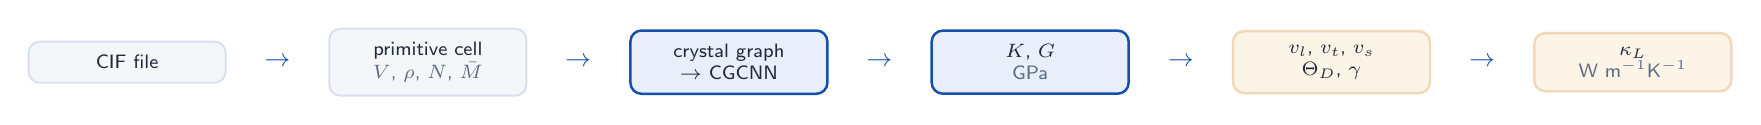
\begin{tikzpicture}[node distance=3.6mm,
  box/.style={rounded corners=4pt, fill=CardBg, draw=CardRule, line width=0.7pt,
              text width=2.15cm, align=center, inner sep=5pt,
              font=\sffamily\scriptsize\color{SlideInk}},
  net/.style={rounded corners=4pt, fill=BlueBg, draw=SlideBlue, line width=0.9pt,
              text width=2.15cm, align=center, inner sep=5pt,
              font=\sffamily\scriptsize\color{SlideInk}},
  phys/.style={rounded corners=4pt, fill=AmberBg, draw=AmberRule, line width=0.9pt,
              text width=2.15cm, align=center, inner sep=5pt,
              font=\sffamily\scriptsize\color{SlideInk}},
  arr/.style={font=\color{SlideBlue}\small}]
  \node[box] (a) {CIF file};
  \node[arr, right=of a] (r1) {$\rightarrow$};
  \node[box, right=of r1] (b) {primitive cell\\ {\color{Muted}$V$, $\rho$, $N$, $\bar{M}$}};
  \node[arr, right=of b] (r2) {$\rightarrow$};
  \node[net, right=of r2] (c) {crystal graph\\ $\rightarrow$ CGCNN};
  \node[arr, right=of c] (r3) {$\rightarrow$};
  \node[net, right=of r3] (d) {$K$, $G$\\ {\color{Muted}GPa}};
  \node[arr, right=of d] (r4) {$\rightarrow$};
  \node[phys, right=of r4] (e) {$v_l$, $v_t$, $v_s$\\ $\Theta_D$, $\gamma$};
  \node[arr, right=of e] (r5) {$\rightarrow$};
  \node[phys, right=of r5] (f) {$\kappa_L$\\ {\color{Muted}W m$^{-1}$K$^{-1}$}};
\end{tikzpicture}
\end{center}

\vspace{4pt}
\begin{columns}[T]
\column{0.48\linewidth}
\Card{5.6cm}{BlueBg}{SlideBlue}{%
  \sffamily\footnotesize
  \textbf{Blue --- learned.} The only fitted part of the whole chain. A graph
  network maps structure to two elastic moduli.}
\column{0.48\linewidth}
\Card{5.6cm}{AmberBg}{AmberRule}{%
  \sffamily\footnotesize
  \textbf{Amber --- physics.} Closed form, no free parameters, no fitting.
  Equations 1--8 on the next three slides.}
\end{columns}

\Takeaway{The network never sees a thermal conductivity. Every structural
quantity ($V$, $\rho$, $N$, $\bar{M}$) is read from the CIF, not predicted ---
which is why two of our screens can differ only through $K$ and $G$.}
\end{frame}

% =============================================================================
\begin{frame}
\SlideHeader{02 \textperiodcentered\ THE PHYSICS}{Equations 1--3 --- from moduli to sound}

{\sffamily\scriptsize
The two predicted moduli fix how fast sound travels through the crystal, and
phonon speed is what sets thermal conductivity.}

\vspace{3pt}
\begin{align}
v_l &= \sqrt{\frac{K + \tfrac{4}{3}G}{\rho}}
   &&\text{longitudinal wave speed} \\[3pt]
v_t &= \sqrt{\frac{G}{\rho}}
   &&\text{transverse wave speed} \\[3pt]
v_s &= \left[\frac{1}{3}\left(\frac{1}{v_l^{3}} + \frac{2}{v_t^{3}}\right)\right]^{-1/3}
   &&\text{averaged sound velocity}
\end{align}

\vspace{4pt}
\begin{center}
{\sffamily\scriptsize
\begin{tabular}{@{}lll@{}}
\toprule
symbol & meaning & unit \\
\midrule
$K$ & bulk modulus \emph{(predicted)} & GPa \\
$G$ & shear modulus \emph{(predicted)} & GPa \\
$\rho$ & mass density \emph{(from the CIF)} & g\,cm$^{-3}$ \\
$v_l,\ v_t,\ v_s$ & longitudinal / transverse / averaged sound velocity & m\,s$^{-1}$ \\
\bottomrule
\end{tabular}}
\end{center}

\vspace{3pt}
{\sffamily\scriptsize\color{Muted}
Eq.~3 is a harmonic-type mean over the three acoustic branches --- one
longitudinal, two transverse --- which is why the transverse term carries a
factor of 2.}
\end{frame}

% =============================================================================
\begin{frame}
\SlideHeader{03 \textperiodcentered\ THE PHYSICS}{Equations 4--6 --- Debye temperature and Gr\"uneisen}

\begin{align}
\Theta_D &= \frac{h}{k_B}\left(\frac{3}{4\pi V}\right)^{1/3} v_s
   &&\text{Debye temperature} \\[3pt]
\nu &= \frac{(v_l/v_t)^2 - 2}{2\,(v_l/v_t)^2 - 2}
   &&\text{Poisson's ratio} \\[3pt]
\gamma &= \frac{3\,(1 + \nu)}{2\,(2 - 3\nu)}
   &&\text{Gr\"uneisen parameter}
\end{align}

\vspace{3pt}
\begin{center}
{\sffamily\scriptsize
\begin{tabular}{@{}llllll@{}}
\toprule
sym & meaning & unit & sym & meaning & unit \\
\midrule
$h$ & Planck const. & J\,s & $\Theta_D$ & Debye temp. & K \\
$k_B$ & Boltzmann const. & J\,K$^{-1}$ & $\nu$ & Poisson's ratio & --- \\
$V$ & vol.\ per atom \emph{(CIF)} & \AA$^3$ & $\gamma$ & Gr\"uneisen & --- \\
\bottomrule
\end{tabular}}
\end{center}

\vspace{1pt}
{\sffamily\scriptsize
\textbf{Eq.~6 matters most:} $\gamma$ is \emph{derived} from the same $K$, $G$.}
\end{frame}

% =============================================================================
\begin{frame}
\SlideHeader{04 \textperiodcentered\ THE PHYSICS}{Equations 7--8 --- two routes to \texorpdfstring{$\kappa_L$}{kappa}}

\begin{align}
\kappa_L^{\text{Slack}} &=
  \frac{A(\gamma)\,\bar{M}\,V^{1/3}\,\Theta_D^{3}}{\gamma^{2}\,T\,N},
  \qquad A(\gamma) = \frac{2.43\times10^{-8}}{1 - \dfrac{0.514}{\gamma} + \dfrac{0.228}{\gamma^{2}}} \\[4pt]
\kappa_L^{\text{cal}} &=
  \frac{G\,v_s\,V^{1/3}}{N\,T}\;e^{-\gamma}
  \qquad\text{\sffamily\scriptsize (PINK Eq.~2 --- three-phonon, $\delta = 1$)}
\end{align}

\vspace{2pt}
\begin{center}
{\sffamily\scriptsize
\begin{tabular}{@{}lll@{}}
\toprule
symbol & meaning & unit \\
\midrule
$\bar{M}$ & mean atomic mass & amu \\
$N$ & atoms per unit cell & --- \\
$T$ & temperature, fixed at 300 & K \\
$A(\gamma)$ & Slack's empirical prefactor & --- \\
$\kappa_L$ & lattice thermal conductivity & W\,m$^{-1}$\,K$^{-1}$ \\
\bottomrule
\end{tabular}}
\end{center}

\vspace{2pt}
{\sffamily\scriptsize
Both are implemented in \texttt{07\_predict\_kappa.py} and checked against the
paper's own released code. \textbf{This project reports $\kappa_L^{\text{cal}}$},
so note its $\gamma$ dependence is \emph{exponential} --- not the $\gamma^{-2}$
of the Slack form. Substituting a different $\gamma$ rescales it by
$e^{\gamma_{\text{old}} - \gamma_{\text{new}}}$.}
\end{frame}

\PartSlide{TWO}{From CIF to two graphs}{Computed from the real NaCl file, not sketched}

% =============================================================================
\begin{frame}
\SlideHeader{05 \textperiodcentered\ CIF TO GRAPH}{NaCl, all the way through}

\begin{center}
\includegraphics[width=0.98\linewidth]{figures/nacl_alignn_graphs.png}
\end{center}

\vspace{-2pt}
{\sffamily\scriptsize
Generated by \texttt{make\_pink\_figures.py} from \texttt{nacl.cif} at
\textbf{ALIGNN's own graph settings} --- cutoff 5.0 \AA, max 12 neighbours,
read from the trained model's config rather than chosen for the picture.
Projection is isometric: in rock salt every $(x,y)$ holds both a Na and a Cl
differing only in $z$, so a flat projection hides one species entirely.}
\end{frame}

% =============================================================================
\begin{frame}
\SlideHeader{06 \textperiodcentered\ CIF TO GRAPH}{What the three panels cost}

\begin{columns}[T]
\column{0.46\linewidth}
{\sffamily\footnotesize
The counts on the previous slide are computed, and they show why the line graph
is the expensive half of ALIGNN:}

\vspace{5pt}
{\sffamily\small
\begin{tabular}{@{}lr@{}}
\toprule
NaCl, one unit cell & \\
\midrule
atoms (nodes of $\mathcal{G}$) & 8 \\
bonds (edges of $\mathcal{G}$) & 96 \\
\textbf{angles (edges of $\mathcal{L}$)} & \textbf{528} \\
\bottomrule
\end{tabular}}

\vspace{6pt}
{\sffamily\footnotesize
Each atom keeps its 12 nearest neighbours, so it contributes 12 bond-nodes and
$\binom{12}{2} = 66$ angle edges. Over 8 atoms that is $8 \times 66 = 528$ ---
\textbf{5.5$\times$ more edges than the atom graph has}.}

\column{0.50\linewidth}
\Card{6.0cm}{CardBg}{CardRule}{%
  \sffamily\footnotesize
  \textbf{Why promote bonds to nodes at all}\\[3pt]
  A message-passing layer updates a node from its neighbours. On the atom graph
  the only geometric quantity a message can carry is the bond \emph{length} ---
  an angle belongs to a \emph{pair} of bonds, and there is nowhere on
  $\mathcal{G}$ for it to live.\\[3pt]
  In $\mathcal{L}$ a pair of bonds \emph{is} an edge, and an edge is exactly
  where a feature attaches.}

\vspace{5pt}
{\sffamily\scriptsize\color{Muted}
Angles enter as $\cos\theta_{jik}$ on a radial basis, the same way distances do
--- smooth where it matters, no discontinuity at $0$ or $\pi$.}
\end{columns}

\Takeaway{Shear modulus is a bond-\emph{bending} property. CGCNN infers it from
lengths alone; ALIGNN is handed the angles directly.}
\end{frame}

\PartSlide{THREE}{Figures 4, 5 and Table 1}{The data, the fit, and the measured check}

% =============================================================================
\begin{frame}
\SlideHeader{07 \textperiodcentered\ FIGURE 4}{Dataset statistics}

\begin{center}
\includegraphics[width=0.72\linewidth]{figures/pink_fig4_dataset_stats.png}
\end{center}

\vspace{-3pt}
{\sffamily\scriptsize
\textbf{Each panel is titled with the population it describes.} A/B use the 1{,}213
CIFs we hold; the 10{,}987 training \emph{structures} are not available offline,
so C/D use formulas and atom counts. Cubic dominates, as in the paper.}
\end{frame}

% =============================================================================
\begin{frame}
\SlideHeader{08 \textperiodcentered\ FIGURE 5}{Predicted vs DFT --- the moduli}

\begin{columns}[T]
\column{0.49\linewidth}
\begin{center}
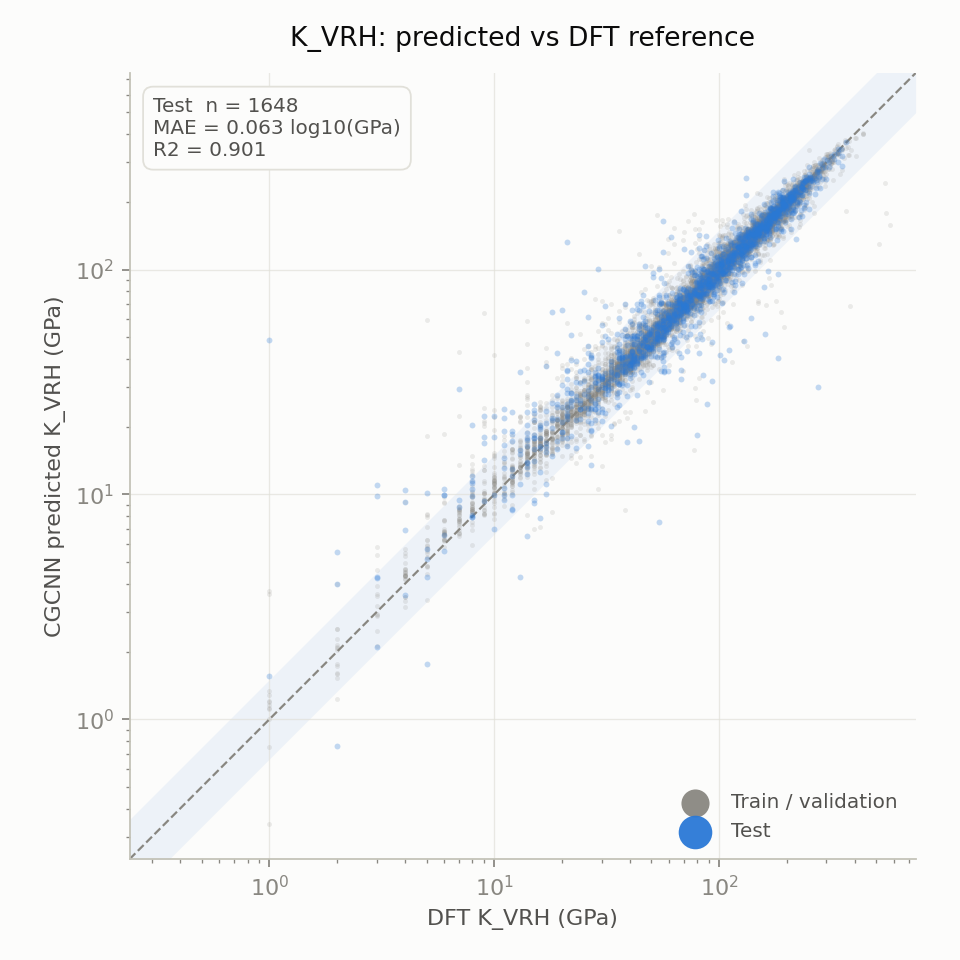
\includegraphics[width=\linewidth]{../results/cgcnn/parity_K_VRH_ens.png}
\end{center}
\column{0.49\linewidth}
\begin{center}
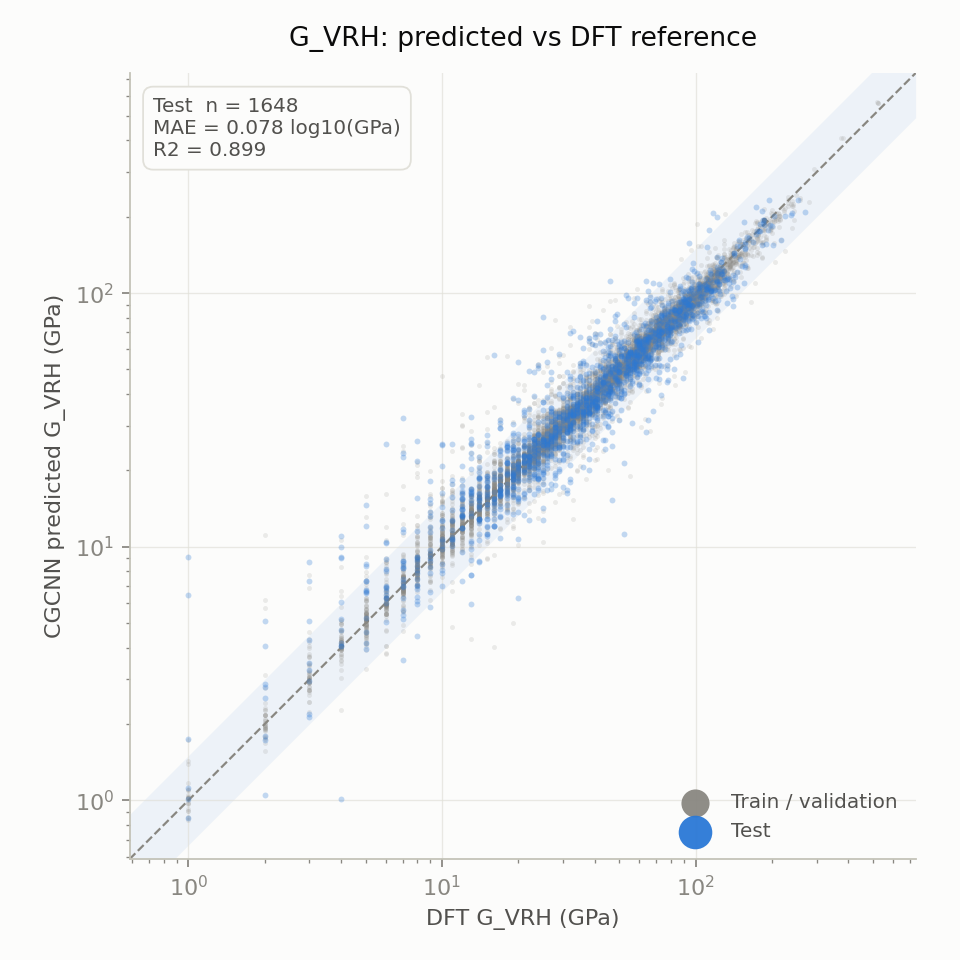
\includegraphics[width=\linewidth]{../results/cgcnn/parity_G_VRH_ens.png}
\end{center}
\end{columns}

\vspace{2pt}
{\sffamily\scriptsize
Our 3-model ensemble on 1{,}648 held-out crystals. Bulk $R^2 = \KEnsRtwo$,
MAE $\KEnsGpa$ GPa; shear $R^2 = \GEnsRtwo$, MAE $\GEnsGpa$ GPa.

\vspace{2pt}
\textbf{These are our numbers, not the paper's.} PINK reports $R^2 = 0.910$ /
MAE $12.926$ for bulk and $R^2 = 0.846$ / MAE $9.263$ for shear on its own test
split. Ours are a different split of a different size --- close, and not the
same experiment.}
\end{frame}

% =============================================================================
\begin{frame}
\SlideHeader{09 \textperiodcentered\ TABLE 1}{45 materials with measured \texorpdfstring{$\kappa_L$}{kappa}}

\begin{columns}[T]
\column{0.54\linewidth}
\begin{center}
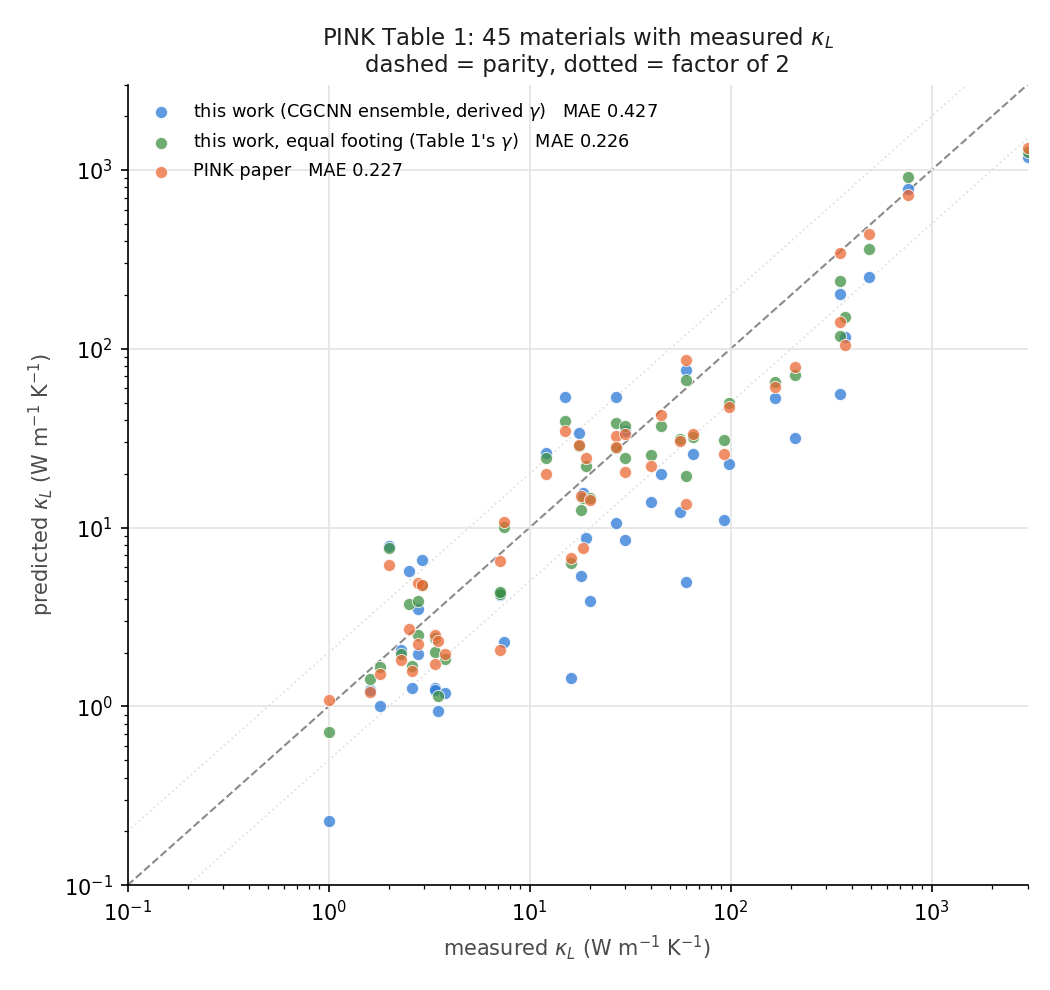
\includegraphics[width=\linewidth]{../results/cgcnn/63_experimental_vs_predicted.png}
\end{center}
\column{0.42\linewidth}
{\sffamily\footnotesize
The paper's Table 1 lists 46 materials with \textbf{experimentally measured}
$\kappa_L$; 45 survive (mp-3490/GaP is deprecated in Materials Project).}

\vspace{5pt}
\Card{5.0cm}{CardBg}{CardRule}{%
  \sffamily\scriptsize
  \textbf{mean $|\Delta \log_{10}|$}\\[3pt]
  ours, derived $\gamma$ \dotfill 0.427\\
  ours, equal footing \dotfill \textbf{0.226}\\
  the PINK paper \dotfill 0.227}

\vspace{5pt}
{\sffamily\scriptsize
Table 1's $\gamma$ comes from AFLOW/experimental lookups, not from Eq.~6. Using
Eq.~6 on both sides --- equal footing --- we match the paper.
\texttt{results/cgcnn/63\_experimental\_vs\_predicted.csv}, 45 rows,
27 columns.}
\end{columns}
\end{frame}

\PartSlide{FOUR}{Figures 6, 7 and 8}{Validation, the funnel, and what came out of it}

% =============================================================================
\begin{frame}
\SlideHeader{10 \textperiodcentered\ FIGURE 6}{\texorpdfstring{$\kappa_L$}{kappa} against an independent pipeline}

\begin{columns}[T]
\column{0.52\linewidth}
\begin{center}
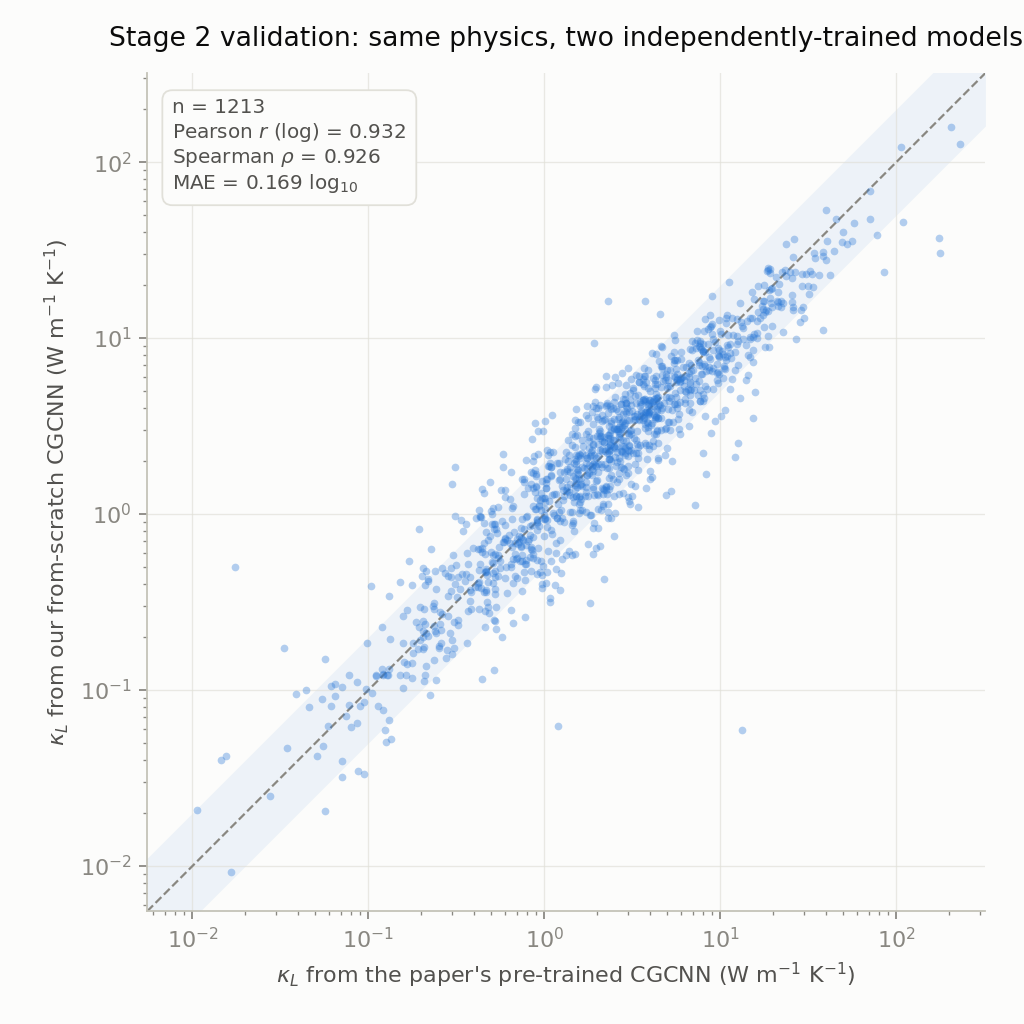
\includegraphics[width=\linewidth]{../results/cgcnn/kappa_validation.png}
\end{center}
\column{0.44\linewidth}
{\sffamily\footnotesize
Our $\kappa_L$ against the paper's own pretrained pipeline on the same 1{,}213
crystals: Pearson $r = 0.932$, Spearman $\rho = 0.926$.

\vspace{4pt}
The equivalent architecture check --- ALIGNN's moduli through the
\emph{unchanged} physics --- agrees even more tightly with our CGCNN ensemble:
$r = 0.940$, $\rho = 0.947$.}

\vspace{5pt}
\Card{5.2cm}{CardBg}{CardRule}{%
  \sffamily\scriptsize
  Two independently trained architectures, sharing only the data, the split and
  Equations 1--8, converging this closely is evidence the pipeline finds
  physical signal rather than architecture-specific noise.}
\end{columns}
\end{frame}

% =============================================================================
\begin{frame}
\SlideHeader{11 \textperiodcentered\ FIGURE 7}{The screening funnel}

\begin{center}
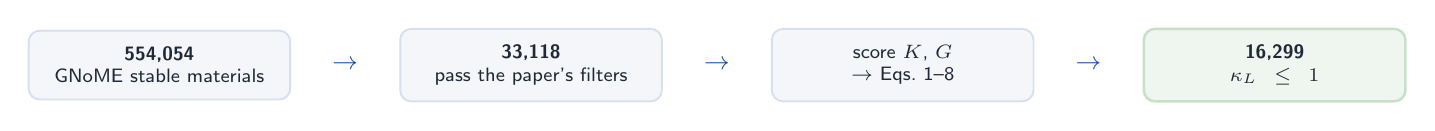
\begin{tikzpicture}[node distance=4mm,
  box/.style={rounded corners=4pt, fill=CardBg, draw=CardRule, line width=0.7pt,
              text width=2.9cm, align=center, inner sep=6pt,
              font=\sffamily\scriptsize\color{SlideInk}},
  hit/.style={rounded corners=4pt, fill=GreenBg, draw=GreenRule, line width=0.9pt,
              text width=2.9cm, align=center, inner sep=6pt,
              font=\sffamily\scriptsize\color{SlideInk}},
  arr/.style={font=\color{SlideBlue}\small}]
  \node[box] (b1) {\textbf{554{,}054}\\ GNoME stable materials};
  \node[arr, right=of b1] (a1) {$\rightarrow$};
  \node[box, right=of a1] (b2) {\textbf{33{,}118}\\ pass the paper's filters};
  \node[arr, right=of b2] (a2) {$\rightarrow$};
  \node[box, right=of a2] (b3) {score $K$, $G$\\ $\rightarrow$ Eqs.\ 1--8};
  \node[arr, right=of b3] (a3) {$\rightarrow$};
  \node[hit, right=of a3] (b4) {\textbf{16{,}299}\\ $\kappa_L \leq 1$};
\end{tikzpicture}
\end{center}

\vspace{5pt}
\begin{columns}[T]
\column{0.48\linewidth}
{\sffamily\footnotesize
\textbf{The paper's funnel reads}
377{,}221 $\rightarrow$ 30{,}199 $\rightarrow$ 26{,}305 $\rightarrow$ 11{,}869.
Ours starts from a larger number because the GNoME snapshot grew after
publication --- stated rather than glossed, because it means the two candidate
lists are not directly comparable.}
\column{0.48\linewidth}
\Card{5.6cm}{CardBg}{CardRule}{%
  \sffamily\footnotesize
  \textbf{70.8\%} of the paper's own 11{,}869 published candidates also appear
  in our independently derived list.\\[3pt]
  {\color{SlideAmber}Flagged: that figure predates several later corrections
  and should be recomputed before publication.}}
\end{columns}
\end{frame}

% =============================================================================
\begin{frame}
\SlideHeader{12 \textperiodcentered\ FIGURE 8}{What the candidates look like}

\begin{columns}[T]
\column{0.49\linewidth}
\begin{center}
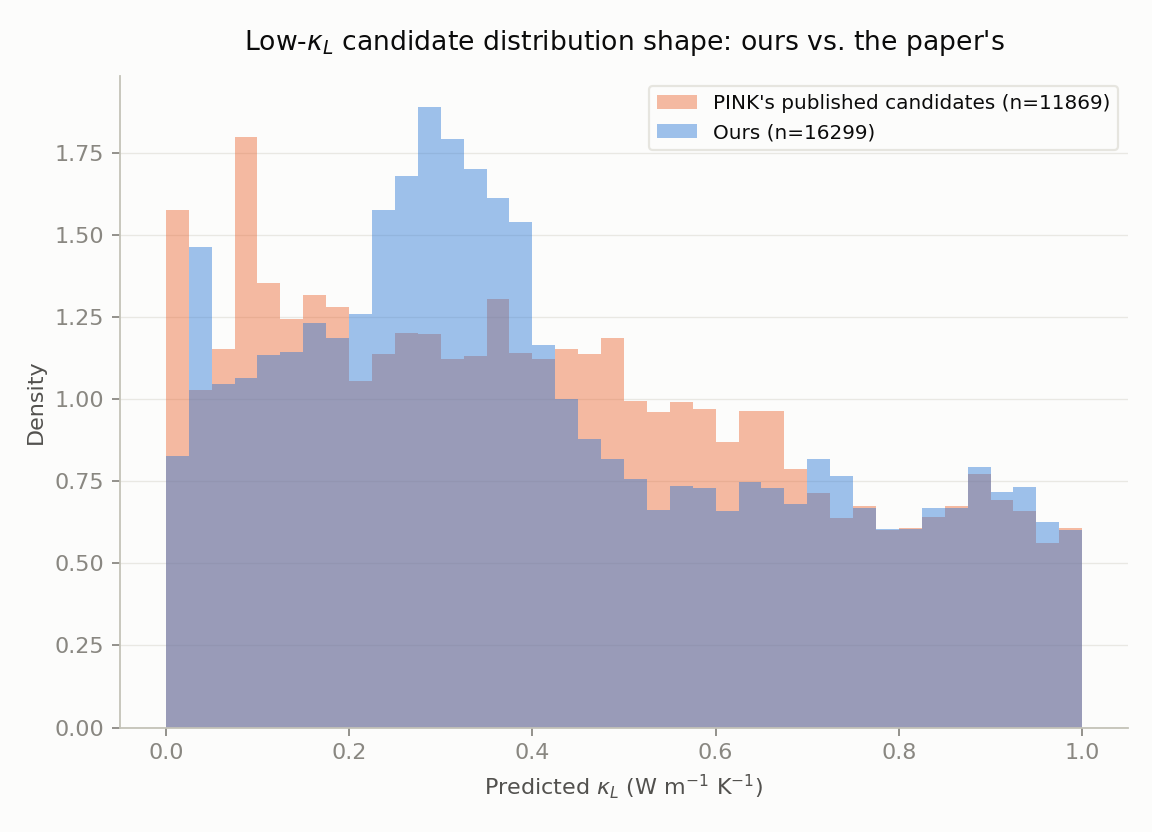
\includegraphics[width=\linewidth]{../results/cgcnn/gnome_kappa_distributions.png}
\end{center}
{\sffamily\scriptsize\color{Muted}\centering A\quad $\kappa_L$ distribution, ours vs the paper's}
\column{0.49\linewidth}
\begin{center}
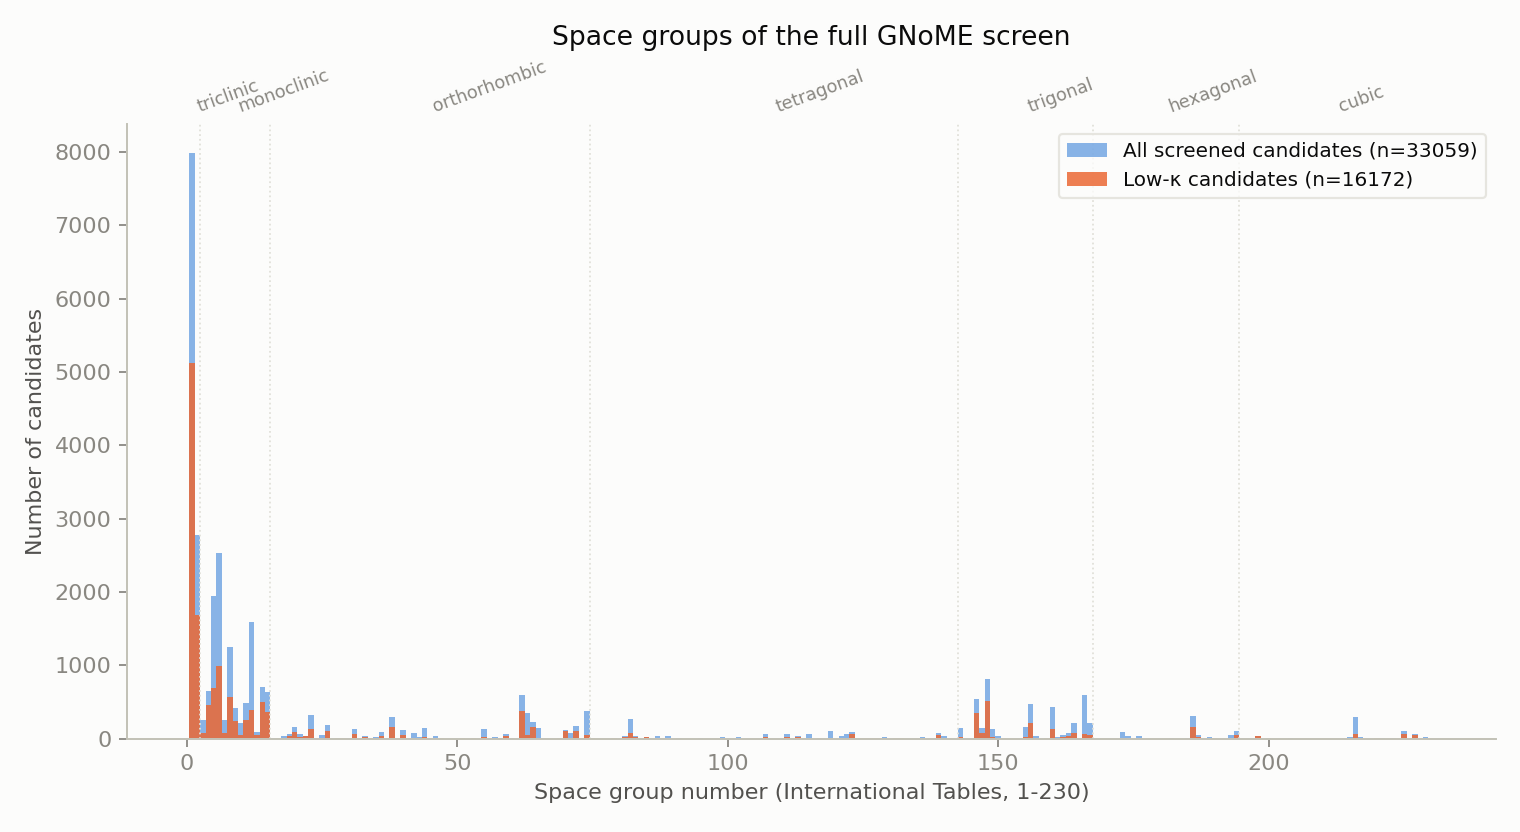
\includegraphics[width=\linewidth]{../results/cgcnn/gnome_screen_spacegroups.png}
\end{center}
{\sffamily\scriptsize\color{Muted}\centering B\quad space groups of the screened pool}
\end{columns}

\vspace{3pt}
{\sffamily\scriptsize
Both distributions span the same range and peak in the same place. Our
candidate set is somewhat more concentrated around
0.25--0.4~W\,m$^{-1}$K$^{-1}$.}
\end{frame}

\PartSlide{FIVE}{Classification of the screen}{By element, symmetry, family, and what we chose for DFT}

% =============================================================================
\begin{frame}
\SlideHeader{13 \textperiodcentered\ CLASSIFICATION}{Elements, against electronegativity}

\begin{center}
\includegraphics[width=0.86\linewidth]{figures/pink_elements_electroneg.png}
\end{center}

\vspace{-3pt}
{\sffamily\scriptsize
Enrichment is the rate at which candidates containing an element are called
low-$\kappa$, divided by the base rate. Above 1.0 the element prefers the
low-$\kappa$ set. \textbf{Halogens sit high and to the right; oxygen sits
lowest} --- heavy soft halide lattices against tight oxide bonding, which is
what Equations 1--3 predict, since a low $G$ means a low $v_s$ means a low
$\kappa_L$.}
\end{frame}

% =============================================================================
\begin{frame}
\SlideHeader{14 \textperiodcentered\ CLASSIFICATION}{Structural families}

\begin{center}
\includegraphics[width=0.92\linewidth]{figures/families_classification.png}
\end{center}

\vspace{-3pt}
{\sffamily\scriptsize
From \texttt{results/families/40\_family\_summary.csv}. Non-oxides dominate the
screen and have by far the highest hit rate; complex 5-element oxides are
numerous but almost never low-$\kappa$ --- \textbf{33 of 3{,}296}. GNoME's
discovered materials skew toward complex, previously uncatalogued
compositions, so simple stoichiometries are largely absent.}
\end{frame}

% =============================================================================
\begin{frame}
\SlideHeader{15 \textperiodcentered\ CLASSIFICATION}{The DFT validation set}

\begin{center}
\includegraphics[width=0.90\linewidth]{figures/dft_validation_set.png}
\end{center}

\vspace{-3pt}
{\sffamily\scriptsize
18 materials, three arms, all $\leq$ 10 atoms.
\textbf{A} consensus low (all four models agree) \textbf{B} adjudication (three
say low, round 9 says high --- these settle a disagreement nothing else can)
\textbf{C} negative control (all four say stiff). Start with
\textbf{MoBr$_5$Cl}: 7 atoms, $Cm$, ALIGNN 0.028 against round 9's 4.524.}
\end{frame}

% =============================================================================
\begin{frame}
\SlideHeader{16 \textperiodcentered\ COMPARISON}{Every model this project has trained}

\begin{center}
\includegraphics[width=0.86\linewidth]{figures/model_comparison.png}
\end{center}

\vspace{-3pt}
{\sffamily\scriptsize
Bars are absent where a model was never trained on that dataset --- not zero,
not measured. \textbf{The composition-only tree beats the CGCNN on AFLOW}
(0.0592 vs 0.1154) while losing on matbench; that is underfitting, not a
limit of graph networks --- the network's \emph{training} error on AFLOW
(0.103) exceeds the tree's \emph{test} error.}
\end{frame}

% =============================================================================
\begingroup
\setbeamercolor{background canvas}{bg=Navy}
\begin{frame}[plain]
\vspace{0.9cm}
\begin{center}
{\color{SlideAmber}\bfseries\sffamily\large FIGURES 9 AND 10}\\[8pt]
{\color{white}\bfseries\headingfont\fontsize{25}{30}\selectfont
  What we cannot reproduce}\\[12pt]
\begin{minipage}{0.80\linewidth}
{\color{Subtle}\sffamily\footnotesize
The paper's last two figures are \textbf{DFT phonon calculations} on
Ag$_3$Te$_4$X --- the primitive structures, phonon dispersions, and then
$\kappa_L$ against temperature, cumulative $\kappa_L$, specific heat, mode group
velocities, scattering phase space and scattering rates.\\[8pt]
Producing them needs a full DFT plus finite-displacement phonon workflow with
\textbf{third-order force constants}, on materials this project has never
computed. That is days of DFT per material and an entirely different toolchain
from anything here.\\[8pt]
{\color{white}No stand-in is drawn for them.} They are the same missing
ground-truth gap the 18-material DFT validation set exists to start closing ---
and the elastic tensors in that set are the cheap first step toward exactly
this kind of calculation.}
\end{minipage}
\end{center}
\end{frame}
\endgroup

\end{document}
